\documentclass[12pt]{article}
\usepackage[a4paper, hmargin={2.8cm, 2.8cm}, vmargin={2.5cm, 2.5cm}]{geometry}
\usepackage{eso-pic} % \AddToShipoutPicture

\usepackage[utf8]{inputenc}
\usepackage[T1]{fontenc}
\usepackage{lmodern}
\usepackage[english]{babel}
\usepackage{cite}
\usepackage{amssymb}
\usepackage{amsfonts}
\usepackage{amsmath}
\usepackage{enumerate}
\usepackage{mathrsfs}
\usepackage{fullpage}
\usepackage[linkcolor=red]{hyperref}
\usepackage[final]{graphicx}
\usepackage{color}
\usepackage{listings}
\renewcommand*\lstlistingname{Code Block}
\definecolor{bg}{rgb}{0.95,0.95,0.95}

%caption distinct from normal text
\usepackage[hang,small,bf]{caption}
\usepackage{hyperref}

\hypersetup{
    colorlinks,%
    citecolor=black,%
    filecolor=black,%
    linkcolor=black,%
    urlcolor=black
}

\author{
  \texttt{Gruppe: 3D} \\
  \texttt{Mikkel Enevoldsen} \\[.4cm]
  \texttt{Kristian Høi} \\[.4cm]
  \texttt{Dominique Chancelier} \\[.4cm]
  \texttt{Carsten Jensen} \\[.4cm]
  Instruktor: Jesper Lundsgaard
  \vspace{8cm}
}

\title{
  \vspace{3cm}
  \Huge{Opgave 5} \\[.25cm]
  \large{Kontekstuel Analyse}
  \vspace{.75cm}
}

\begin{document}

\AddToShipoutPicture*{\put(0,0){\includegraphics*[viewport=0 0 700 600]{includes/ku-farve}}}
\AddToShipoutPicture*{\put(0,602){\includegraphics*[viewport=0 600 700 1600]{includes/ku-farve}}}

%% Change `ku-en` to `nat-en` to use the `Faculty of Science` header
\AddToShipoutPicture*{\put(0,0){\includegraphics*{includes/ku-en}}}

\clearpage\maketitle
\thispagestyle{empty}

\newpage

\tableofcontents %generate table of content

\thispagestyle{empty}

\newpage
\pagestyle{plain}
\setcounter{page}{1}
\pagenumbering{arabic}

\section{Fremgangsmåde}
Vores generelle fremgangsmåde var at, gennemføre en brainstorm og itnerviews før vi begyndte, at definere hvad vores fiva app skulle understøtte af funktioner. Til vores interview udarbejdede vi en tjekliste, hvorpå vi havde en strukturet fremgangsmåde under de interviews.\\
Først lavede vi en PACT analyse, hvor vi prøvede at danne os et overblik over domænet. Dvs. hvilke personer forventer vi at bruge appen i hvilken kontekst og med hvilken teknologi tænkes de at bruge.\\

Med henblik på interviews fandt vi vores deltager på gaden, hvor vi spurgte handlede ved supermarkeder hvor vi spurgte dem om det fremtidige system.\\
Kønsopdelingen for interviewdeltagerne er 3 mænd og 3 kvinder. nedenunder:
\begin{center}
    \begin{tabular}{ |l | l | l | l | l |}
    \hline
    \textbf{Nr.} & \textbf{Køn} & \textbf{alder} & \textbf{uddannelse} & \textbf{Arbejde}\\ \hline
    1 & Mand & 67 & Kok & Pensionist \\ \hline
    2 & Kvinde & 31 & RUC & Journalist \\ \hline
    3 & Mand & 68 & Klejnsmed & Pensionist \\ \hline
    4 & Kvinde & 23 & Medie-videnskab & Studerende \\ \hline
    5 & Mand & 19 & HTX & Studerende \\ \hline
    6 & Kvinde & 41 & Erhversøkonomi og mediekutlur & Arbejdsløs \\ \hline
     \end{tabular}
\end{center}
På baggrund af interviews og brainstorming kunne vi begynde at udforme hvilke funktioner vores system skulle ud og hvilke hensyn vi skulle tag til de fremtidige brugere af produktet.\\
På baggrund af vores analyse med interview og brainstorm udarbejde vi en målgruppe og to scenarier, hvor vi prøvede at forstille os et muligt forløb af interaktion mellem system og brugeren, hvor mest fokuserede på brugerens synsvinkel, da implementationsdetajler ikke kan laves på nuværende stadie\\
Tilsidst kunne vi lave vores papirs-prototype for at give os et overblik over
Til vores interview har vi spurgt seks personer. 
\newpage
\section{Resultat af indledende PACT-analyse}
Vi indledte projektet med brainstorm med udgangspunkt i applikationen FIVA(Finde vare i supermarkedet). Af den process fik vi nogle stikord, som vi tager udgangspunkt i til bearbejdning af vores første interview tjekliste.\\
 
\noindent \textbf{People}
\begin{itemize} 
\item Sprogforskelle hvilke sprog synes vil være passende for FIVA
\item Hukommelse 
\item Generthed (sociale udfordringer ved henvendelse om vareplacering)
\item Socialklasser (indkomstforskelle)
\item Indkøbserfaring\\
\end{itemize}

\noindent Gennem brainstorming af People-delen af PACT-analysen, kom vi frem til ovenstående punkter. Vi mener at det er relevant at diskutere FIVA-appens sprogvalg, da der, specielt i multikulturelle områder, kan være relevant med andet end dansk. Appen kunne rettes mod glemsomme brugere, der ville kunne udnytte at have deres indkøbsseddel på smartphone i stedet for at skulle huske en fysisk seddel. Derudover kan appen hjælpe folk, der generelt finder det grænseoverskridende at spørge medarbejdere om hjælp. Vi diskuterede yderligere hvorvidt socialklasse- og indkomstforskelle samt hvor erfarne indkøbere brugerne er kunne have en relevans.\\

\noindent \textbf{Activity} 
\begin{itemize}
\item Hyppighed 
\item Indkøbsfrekvens  
\item Tidspres
\item Formålet veldefineret: Handle ind.
\item Præventivt varetjek.\\
\end{itemize}

\noindent Vi brainstormede med udgangspunkt i at den hovedsagelige opgave er at købe ind, hvori der er forbundet forskellige aspekter. Det kunne være hvor mange gange en kunde handler ind om dagen, og indkøbsturene er presset tidsmæssigt. Yderligere kunne en mulighed for at tjekke varens status og placering før indkøbsturen startede også blive relevant.\\

\newpage

\noindent \textbf{Context}
\begin{itemize}
\item Supermarkeder - indkøb\\
\end{itemize}

\noindent Det åbenlyse miljø, hvor FIVA-appen kan blive aktuel, er i supermarkeder i forbindelse med indkøb og navigation i en sådan butik.\\

\noindent \textbf{Technology}
\begin{itemize}
\item Smartphone 
\item GPS-tilgængelighed
\item Hurtighed
\item Højtlæsning af resultater\\
\end{itemize}

\noindent Den primære anvend teknologi er en smartphone, som har nogle indbyggede features, der ville kunne bruges til en sådan app. Det kunne eksempelvis være smartphonens GPS, som kan hjælpe brugerne med at finde deres varer i stil med andre GPS-applikationer. Vi forestiller os at et afgørende element er, hvor hurtigt FIVA-appen vil kunne finde en vare for brugeren. Vi overvejede yderligere muligheden for højtlæsning af resultater og navigationen.
   
\newpage

\section{Tjekliste til interview}
\textbf{Introduktion}\\
"Vi er datalogistuderende fra Københanvs Universitet, som skal designe en applikation omhandlende at gøre det lettere for kunden at finde varer. Vi ønsker at bruge 10 minutter på at få dine tanker omkring en sådan applikation  i et interview."
 
\begin{enumerate}
\item Fakta
\begin{enumerate}
\item Observér: Køn
\item Hvor gammel er du?
\item Hvilken teknologisk erfaring har du? Bruger du smartphone på daglig basis?
\end{enumerate}

\item Socialklasse "Hvilket erhverv og/eller uddannelsesbaggrund har du?"

\item Indkøbsfrekvens "Hvor tit handler du ind - og i hvilket tidsrum?"

\begin{enumerate}
\item Erfaring	"På hvilket niveau, erfaringsmæssigt, vil du beskrive dig selv som indkøber?"
\end{enumerate}

\item Tidsfaktor "Hvor lang tid har du til rådighed, når du handler ind?"
\item Motivation "Hvilken tilgang har du til indkøb - har du eksempelvis en struktureret plan over varer, eller køber du hvad der falder dig ind?"
\item Vareplacering "Fortæl mig om en situation, hvor du ikke har kunnet kunne finde en vare i et supermarked."

\begin{enumerate}
\item Hjælp "Hvor ofte må du spørge en medarbejder efter hjælp?"
\item Medarbejderfravær "Hvad gør du, når du ikke kan finde en varer og ikke kan komme i kontakt med en medarbejder?"
\end{enumerate}

\item Medarbejderkonfrontation "Hvilke udfordringer forbinder du med at skulle opsøge en medarbejder om en vares placering?"
\item Hukommelse "Hvor mange gange om måneden glemmer du hvad du skal købe i et supermarked? - Kan du fortælle om en specifik situation?"
\item Teknologisk vane "Hvis du har en smartphone, hvordan bruger du så den i forbindelse med indkøb?"

\begin{enumerate}
\item Teknologisk til-/fravalg "Hvorfor foretrækker du smartphone frem for andre alternativer?"
\end{enumerate}

\item Forberedelse "Hvordan forbereder du dig på en indkøbstur?"

\begin{enumerate}
\item Præventivt varetjek "Hvis vi kigger på de sidste 100 gange du har skullet købe ind, hvor mange gange vil du skyde på at du har ringer og spurgt i forvejen om de har en vare?"
\end{enumerate}

\item Forventning "Hvad ville du forvente en sådan applikation skulle indeholde? Og hvad må den absolut ikke indeholde?"
\item Hurtighed	"Hvor lang tid vil du sige, det højst burde tage at finde en vare ved hjælp af FIVA-appen, hvorfor?"
\item Sprogforskelle "Hvilket sprog synes du FIVA-appen skal være på?"
\item Nødvendighed "Ville du bruge en varelokaliserings-app til din smartphone, hvis sådan en fandtes - hvorfor?"

\begin{enumerate}
\item Alternativer "Kan du komme på alternativer, der ville gøre en sådan applikation overflødig?"
\end{enumerate}

\end{enumerate}

\section{Interviewresultater}
\subsection{Brugernes nuværende oplevelse}
\begin{enumerate}
\item Flere brugere er tidspressede når de skal handle ind, og oplever det derfor stressende, når det tager lang tid, som eksempelvis bruger () finder at det tager at finde specifikke varer.

\item Brugerne oplevede at hjælpen de fik, når de spurgte, ofte tog lang tid og til tidere var utilstrækkelig. Bruger (k,31) oplevede at medarbejder ikke kunne finde en varen og måtte tilkalde yderligere hjælp.

\item Brugere (1,2,3) finder relevansen af FIVA-appen til primært at være i supermarkeder, de ikke kender eller har handlet ind i før. De fleste kender placeringen på varerne i supermarkeder de tit kommer i.

\item Bruger (m,68)(k,31)(m,19)(m,67) fandt udfordringer med at konfrontere medarbejdere i forbindelse med placering på varer. Bruger (m,67)(m,68) fandt kontakt til medarbejdere besværlig, fandt dem svære at finde og ønskede ikke at spilde deres tid, mens bruger (k,31) vurderede der kunne være sproglige vanskeligheder hvis medarbejderne ikke taler dansk. Bruger (m, 19) fandt det akavet at spørge om hjælp. Kun en bruger (k, 41) sagde at hun ikke fandt nogen problemer med at spørge medarbejdere. De fleste (bruger 1, 2, 3, 4 og 6) sagde dog, at de på trods af disse udfordringer stadig opsøgte medarbejdere for at finde en vare, selvom det for brugers (()) vedkommende er en situation der kun sjældent forekommer.

\item Den generelle bruger (bruger (k,23)() ) skriver altid en indkøbsliste hjemmefra, som de bruger til at strukturere deres indkøb. Nogle specificerede dog yderligere, og bruger kun en liste ved større indkøbsture. Flere (bruger ()()) bruger ydermere i forvejen deres smartphone til at notere deres indkøbsliste ned på. 

\item Nogle brugere laver ugentligt mange små ture, hvor de kun køber få varer. Dette sker som oftest som konsekvens af tidligere glemt indkøb.

\item Nogle brugere strukturerer nøje deres indkøb efter andre daglige aktiviteter. Bruger (k,41) handler ind flere gange om dagen - en gang før hun afleverer børn i skole, og en gang på vej hjem fra at hente dem.
\end{enumerate}
\subsection{Forventning til appen}
\begin{enumerate}
\item Mange brugere (1,2,3) syntes at FIVA-appen skal kunne lokalisere varer og give de nødvendige direktioner hurtigt og effektivt. De fleste af dem (1,2) mener at det maksimalt må tage 30 sekunder at for appen at vise den korteste rute.

\item En bruger (1) mener at man skal kunne følge sin rute med en live GPS, i stil med den service Google maps eksempelvis tilbyder.\\

\item En bruger siger, at FIVA-appen skal være simpelt sat op og let at bruge. Bruger (1) mener yderligere at den skal indeholde et begrænset antal funktioner, for at gøre appen mere overskuelig og nemmere at arbejde med. 

\item Ifølge flere brugere, ville FIVA-appen skulle indeholde muligheden for at danne en indkøbsliste, og derved kombinere flere valgte varer og udregne en optimal rute for hele indkøbsturen.

\item En bruger (1) mener at appen, af overskuelighedsmæssige årsager, udelukkende skal være på dansk, mens flere andre brugere også synes at appen burde tilbydes på engelsk.

\item Det ville være forstyrende for flere brugere (1,2), hvis appen indeholdte udefrakommende reklamer.

\item En bruger (1) synes at man kunne give appen et socialt medie aspekt, således at brugerne skal kunne interagere med hinanden.

\item En bruger foreslog, at der kunne være en prissammenlignings mulighed inkluderet i appen, så hvis en vare skulle være billigere i et nærtliggende supermarked, skal appen gøre brugeren opmærksom på denne mulighed.

\item Flere brugere mener, at appen skal indeholde en søgefunktion, der når der søges efter varer, skal komme med søgeforslag efterhånden som der tastes ind. Den skal også kunne foreslå mere specifikke varer til en søgning.
\end{enumerate}

\newpage

\section{Kerneopgaver}

\noindent Gruppen har ved hjælp af brainstorming og diskussion yderligere opnået følgende tilføjelser til kerneopgaverne:

\begin{itemize}
\item Appen skal kunne finde varen i butikken og oplyse hyldenummer.
\item Der skal være implementeret en søgefunktion, som skal kunne hjælpe brugeren og automatisk færdiggøre søgning. Derudover skal den kunne bidrage med yderligere hjælp, eksempelvis hvis kunden bare søger på "vin", skal appen komme med forslag til specifikke vine.
\item GPS-navigation i supermarkedet.
\item Appen skal kunne finde det nærmeste supermarked.
\item Det skal være muligt at finde den korteste vej til kassen på hvilket som helst tidspunkt i indkøbsturen.
\end{itemize}

\noindent På basis af en række interviews, er følgende tilføjelser til kerneopgaver relevante.

\begin{itemize}
\item Det skal være muligt at tjekke om en vare er billigere hos nabobutikken. Appen skal kunne sammenligne priser på varer i en radius af omkring 300 meter.
\item Appen skal være simpel, minimalistisk og uden for mange funktioner, der ultimativt vil gøre den lettere at bruge for brugerne.
\item Appen skal indenfor max 20 sekunder kunne finde varer. Det skal yderligere også gå hurtigt at danne en optimal rute rundt i supermarkedet.
\item Appen skal indeholde en indkøbsliste, der skal hjælpe brugeren med at huske varerne de skal købe. Det skal derudover gøre det muligt at danne en optimal rute med en række varer, som i sidste ende går ud ved kassen.
\end{itemize}

\section{M\aa lgrupper og m\aa lgruppebeskrivelse}
\begin{itemize}
\item Kunder, der er vante smartphone-brugere, der ønsker at komme hurtigt igennem indkøb.
\item Kunder, der er vante smartphone-brugere, der handler ind til flere dage.
\item Kunder, der anvender smartphone til simpelt brug, som ønsker at komme ubesværet igennem indkøb.
\item Prisbevidste kunder der ønsker billigere varer.
\end{itemize}

\subsection{Målgruppebeskrivelse}
Målgruppen handler ind 3-4 gange om ugen. De ønsker en let og hurtig indkøbstur, hvor eventuelle problemer hurtigt ville kunne løses gennem FIVA-appen. De ønsker problemfrit at finde varer, som de sjældent køber.\\
Brugerne er vante indkøbere, og kender derfor det forventede varesortiment i butikken de ønsker at handle i.\\

\noindent Målgruppen bruger deres smartphones generelt til normal kommunikation, så som at ringe, sms og internetsøgninger. Brugeren ved hvad applikationer er, og bruger forbrugsapps, som eksempelvis Danske Banks mobilbank, Google Maps og Rejseplanen efter behov.\\

\noindent Målgruppen forstår at bruge en søgefunktion og følge en GPS' angivelser. De ved ikke hvordan smartphonen og appen fungerer internt. For dem er en smartphone, et redskab til at gøre hverdagen lettere.

\section{Personas}

\subsection{Lars Jensen}

Lars Jensen er 57 år og bor i en forstad til Aarhus. Her han boet han sammen med sin kone, Lis Jensen, i de sidste 25 år. Sammen har de to børn, Michael på 18 og Anne på 21, der begge er flyttet hjemmefra.\\

\noindent Lars er uddannet elektriker, og har været vant til at gøre tingene selv i det meste af sit liv. Lars har haft en smartphone i omkring 2 år, og er ved at blive fortrolig med dens smarte funktioner.\\

\noindent Når der skal handles ind, er det oftest konen der sørger for det. Men desværre er Lis' hukommelse ikke hvad den har været, så derfor må Lars af og til ned og købe de enkelte ting hun glemmer. Han synes det er irriterende, at han så ofte må spørge medarbejdere om hjælp til at finde de forskellige varer. Han synes det spilder tiden for begge parter.

\subsection{Maria Møller}

\noindent Maria Møller er 36 år og bor på Vesterbro i København. Hun bor sammen med sin søn, Emil, på 4 år. Maria er uddannet journalist på RUC, og er ansat på dagbladet Information. Hun har haft en smartphone i omkring 7 år og bruger den dagligt til at kommunikere med familie og venner samt tjekke nyheder.\\

\noindent Maria er glad for at udforske forskellige madkulturer, og hendes yndlingskøkkener er det asiatiske eller mexicanske. Dog har hun for nyligt begyndt at blive inspireret af det nynordiske køkken. Derfor handler hun mange forskellige og nye varer, som hun ikke altid ved hvor er i butikken. Derfor må hun ofte spørge medarbejderne om hjælp - og har oplevet flere gange, at de heller ikke ved hvor varen er.

\section{Scenarier}

\subsection{Lars Jensen}
Lars får at vide, at han skal ned og købe fennikel og kaffefiltre. Når Lars ankommer til supermarkedet åbner han sin nye FIVA-app og indtaster fennikel og kaffefilter i søgefunktionen. Lars har nu en rute, som han følger og finder sine varer. Han bruger "Gå til kassen"-funktionen, og får sin rute til kassen. Lars betaler, og skynder sig hjem.

\subsection{Maria Møller}
Maria sidder derhjemme og planlægger sin indkøbsliste. Her bruger FIVA-appen til at indskrive alle sine varer. Når Maria senere på dagen går ned for at handle, åbner hun appen og beder om ruten til sin indkøbsliste. Hun følger sin rute, men kommer undervejs i tanke om at hun også skal have artiskokker, som hun tilfældigvis ikke ved hvor ligger. Hun taster ind i appen, som tilpasser til hendes rute og viser placeringen på artiskokker. Hun finder sine artiskokker, og fortsætter sin rute.

\newpage

\section{Prototype}
\fbox{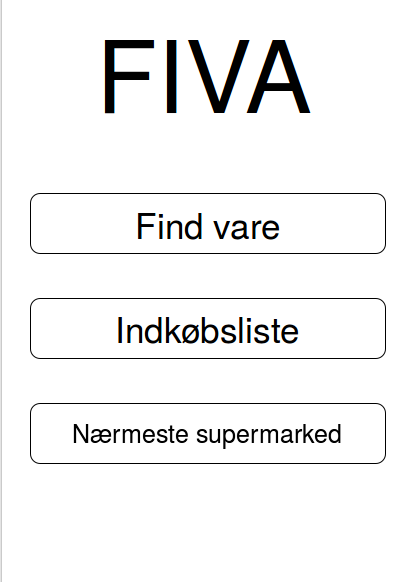
\includegraphics[scale=0.35]{FivaProto/fivaforside.png}} \\
\\
\noindent Find vare undermenu, søgning og navigation til enkelt vares placering:\\

\noindent \fbox{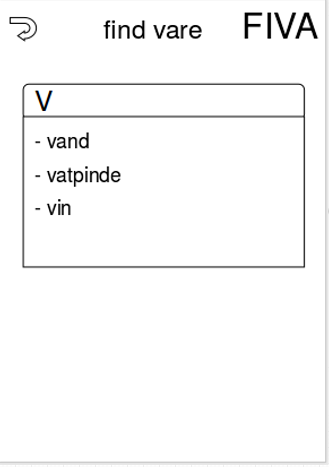
\includegraphics[scale=0.435]{FivaProto/soegauto.png}}
\fbox{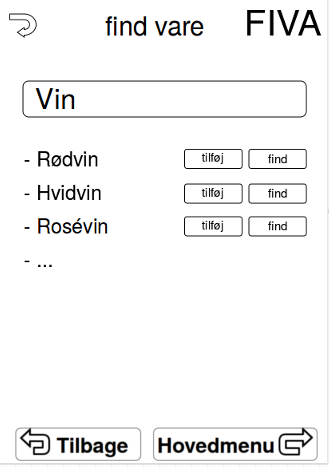
\includegraphics[scale=0.435]{FivaProto/soegeresultat.png}}
\fbox{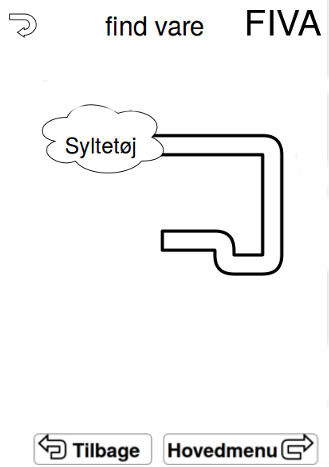
\includegraphics[scale=0.435]{FivaProto/findenkeltvare.png}}

\newpage

\noindent Indkøbsliste og ruten til den pågældende sammensætning af varer:\\

\noindent \fbox{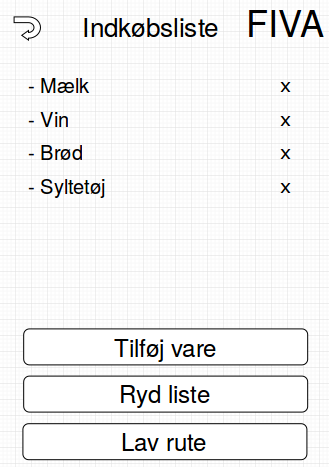
\includegraphics[scale=0.435]{FivaProto/indkoebsliste.png}}
\fbox{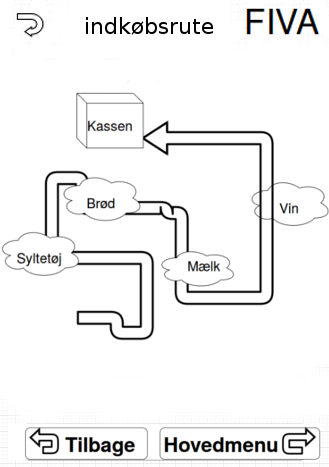
\includegraphics[scale=0.435]{FivaProto/butiksnavigation.png}}\\
\\
\noindent Nærmeste supermarked og navigation hertil:\\

\noindent \fbox{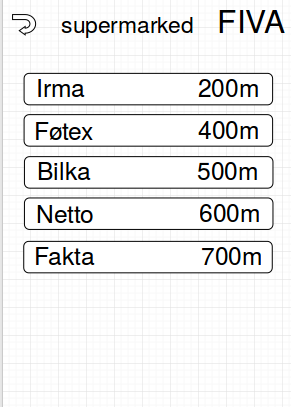
\includegraphics[scale=0.5]{FivaProto/naermestesupermarked.png}}
\fbox{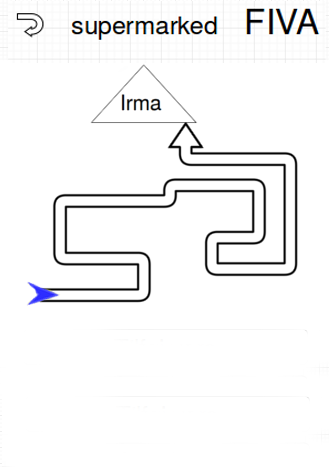
\includegraphics[scale=0.435]{FivaProto/naermsupnavigation.png}}

\newpage

\section{Erfaringer}

Vi har lært, hvor vigtigt det er at lave en grundig research, inden man går i gang med at udvikle en app. Folk ikke ønsker at bruge for lang tid på deres indkøb. Derfor skal app'en være hurtig og brugervenlig, og det skal være muligt at indtaste en indkøbsliste, fordi det er en vigtig del af folks indkøb.

\section{Appendix}

Hvert gruppemedlem har i gennemsnit brugt i omegnen af 20 timer på denne opgave.

\end{document}
